
\documentclass{llncs}
\usepackage{llncsdoc}
\usepackage{graphicx} % Required for the inclusion of images
\usepackage{amsmath} % Required for some math elements 
\usepackage{caption}
\usepackage{url}
\usepackage{algorithmic}
\usepackage{listings}
\usepackage{makeidx}
\usepackage{enumitem}
\usepackage{subfig}

%
\begin{document}

\lstset{numbers=left, basicstyle=\small, numbersep=5pt, numberstyle=\tiny}

\section{Introduction}

rSLA is a domain specific language (DSL) for expressing and managing service level agreements (SLAs) in a cloud environment. rSLA is written with Ruby \cite{ruby}, a dynamic scripting language that enables rapid prototyping and application development. The rSLA DSL is described by an alphabet and by production rules for using and extending the language. The rSLA language framework also provides a runtime engine to deploy and instantly run an rSLA service in a cloud environment.

Cloud service management does not yet support enough automated and transparent solutions for the management of leased resources. There is no established standard so far for the automatic expression and management of SLAs for cloud services.

Although the scientific literature provides plentiful results on the automated management of SLAs for distributed computing \cite{wsla, wsag, more}, cloud markets hesitate to adopt such solutions. Provisioning of cloud services is thus handled either manually or with software tools that do not embrace cloud service characteristics.


The rSLA is deployed on the IBM Bluemix platform as a ruby web service using the sinatra gem. 
The DSL enables the automated generation of customized SLAs and the transparent management of cloud resources.
what problem does it solve? why is it needed?

rSLA provides an alphabet with production rules to express, a runtime engine to run.

How is the paper structured

-what is the problem that the language solves, motivation to solve this problem
-language structure, alphabet, production rules
-language runtime
-current testing, future testing

\section{Problem definition/ motivation}
Cloud service management does not yet support enough automated and transparent solutions for the management of leased resources. 

There is no established standard so far for the automatic expression and management of SLAs for cloud services.

The rSLA language is not intended to be used only by engineers. An important goal in the language design is to provide a high-level, easy to use and to extend tool that is suitable either for human or machine consumption.

\section{rSLA DSL}

alphabet, vocabulary, language structure

production rules


\subsection{rSLA language structure, alphabet}

 point of this subsection?

The rSLA language follows the semantic decomposition of the WSLA specification \cite{wsla}, where an SLA takes the form of a hierarchical tree with a single root node and numerous uni-directional edges. Figure \ref{rSLA_diag} illustrates the rSLA vocabulary as a tree of classes that the rSLA DSL implements. Connections between nodes in the rSLA tree highlight the nesting of SLA context. 

In the rSLA alphabet the root node of an rSLA tree represents an SLA object. In Figure \ref{rSLA_diag} nodes that are positioned close to the root, designate branches of SLA context (e.g. base and composite metrics, service level objectives). Edges between nodes are uni-directed to illustrate the rSLA tree hierarchical schema.

\begin{figure}
  \centering
    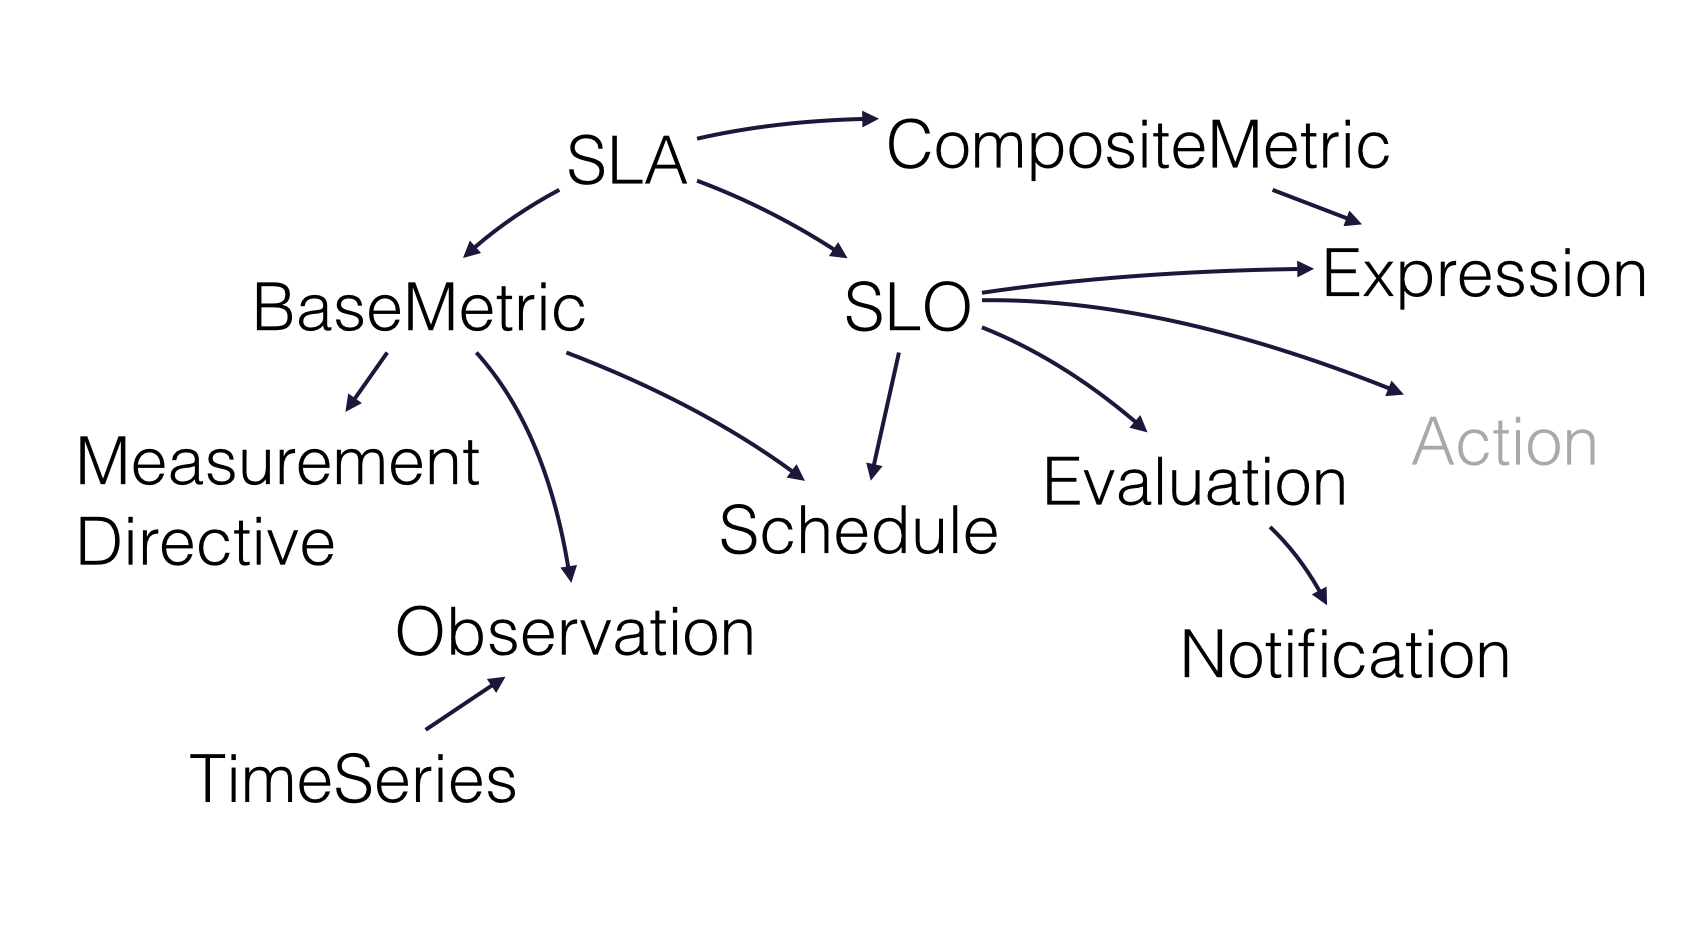
\includegraphics[width=0.5\textwidth]{pics/rslauser}
    \caption{rSLA DSL class diagram}
    \label{rSLA_diag}
\end{figure}

 rSLA supports the creation of programming blocks that express SLA context and that are necessary to run and manage rSLAs in a cloud environment. Listing \ref{lst} describes the rSLA vocabulary using set notation to highlight the nesting between language objects:
\begin{lstlisting}[breaklines, mathescape, firstnumber=auto, caption=rSLA vocabulary, label=lst]
SLA $\supset$ { BaseMetric+, CompositeMetric*, SLO+ }
BaseMetric $\supset$ { MeasurementDirective, Observation*, Schedule* }
CompositeMetric $\supset$ { Expression* }
SLO $\supset$ { Expression*, Action*, Evaluation*, Schedule* }
\end{lstlisting}

In the rSLA language nested relationships denote inclusive associations between objects. For example, an SLA includes base and composite metrics as well as SLOs. Inclusive relationships of rSLA objects do not share same multiplicity rules (listing \ref{lst}). The rSLA DSL follows the WSLA specification \cite{wsla} with respect to the definition of rSLA objects and of their basic attributes.

In Figure \ref{rSLA_diag} the $Notification$ and $TimeSeries$ classes do not appear in the rSLA set representation. These two classes produce objects that help with service level management operations like the statistical analysis of data coming from monitoring or automated notification reports on scheduled events of service level evaluation. Such two classes are not initially required to build and run SLA instances in a cloud environment, but may be required while one or more SLA management tasks are processed.



conclude that
 
\subsection{rSLA language production rules}

rSLA language constructs: elements have relationships/dependencies, there is nesting and management dependencies

production rules

\section{rSLA editing, runtime}
ready to use functions

The rSLA alphabet consists of language elements that require user input for their creation in an rSLA runtime environment. A DSL user can directly edit code-block scripts in ruby, start a cloud rSLA service and create an active SLA object. In the diagram solid black arrows indicate that user-input is required to create the equivalent objects in an rSLA running environment. 

In Figure \ref{rSLA_diag} language elements that require user-input represent tree branches for the creation of service level agreements. DSL user-input requires editing a ruby script to describe the attributes for any new rSLA object. 

The rSLA language also contains elements, whose definition with an rSLA service requires that at least one SLA object exists (ex. base metric, slo). A DSL user can edit the context of such elements and associate them with required objects using code blocks in ruby SLA scripts.

\section{rSLA deployment }
evaluation examples

\bibliography{spec}

%----------------------------------------------------------------------------------------


\end{document}
